\subsection{Die letzten Lebensjahre}

\hypertarget{RefHeadingToc100333738}{}  [Warning: Image ignored]
% Unhandled or unsupported graphics:
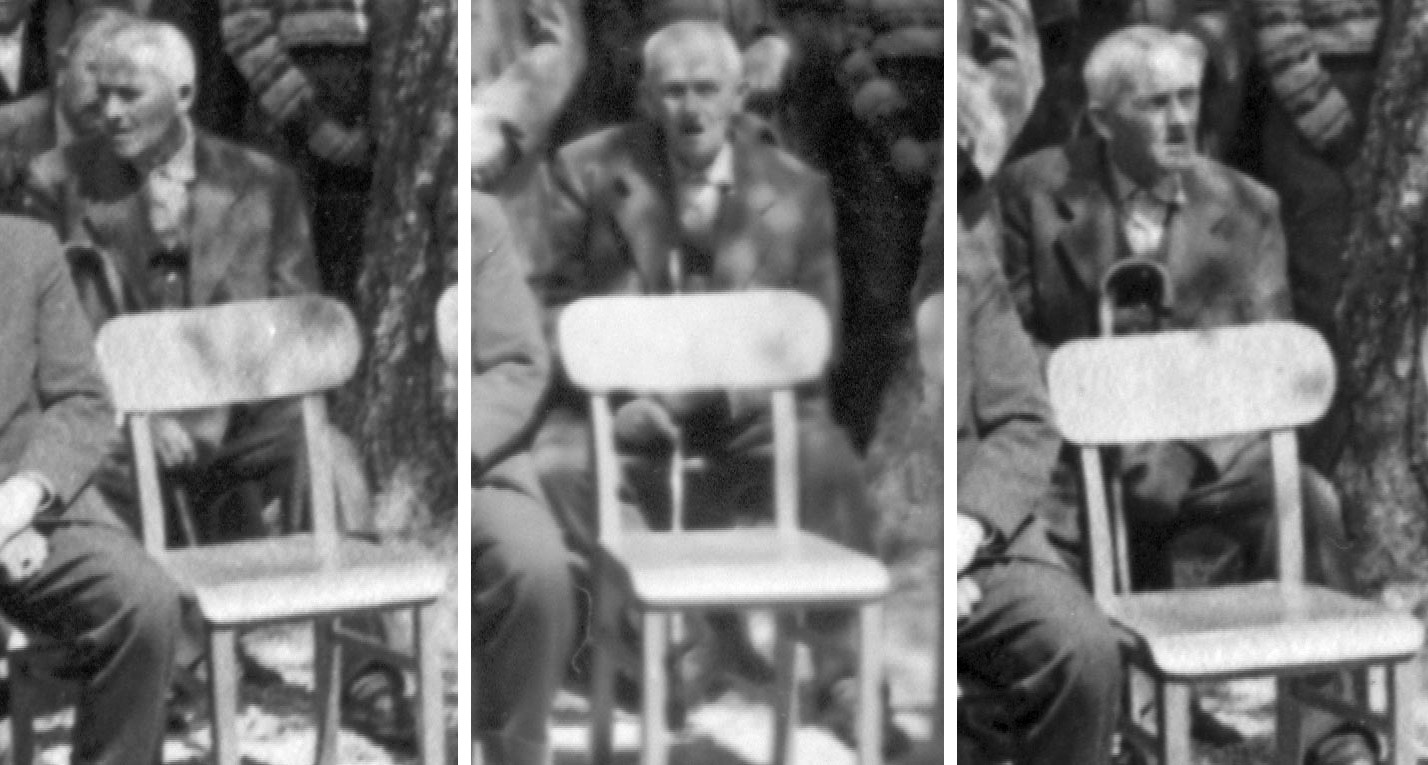
\includegraphics[width=15.981cm,height=8.56cm]{pictures/zulassungsarbeit-img053.jpg}


August Högn auf Bildern, die zur
Einweihung des Schulanbaus an Christihimmelfahrt 1959 aufgenommen
wurden.

Einen tiefen Einschnitt in Högns unruhiges Rentnerleben stellte sein
Schlaganfall Ende 1953 dar. Sein Ruhestand, der eigentlich schon 1945
mit der Suspendierung vom Schuldienst infolge der Entnazifizierung
begann und nur durch einen kurzen Schuleinsatz 1947 \footnote{Dokument
Nr. 48, Zeitungsartikel aus Viechtacher Bayerwald-Bote, 2.8.1958}
unterbrochen wurde, konnte vor 1953 wohl kaum als solcher bezeichnet
werden, wenn man seine Aktivitäten für die Kirche und Heimatkunde
betrachtet.

Vieles spricht dafür, dass Högn trotz seiner körperlichen
Beeinträchtigungen ab 1954 ein aktives Leben führte. Er war sogar noch
schöpferisch tätig, wie sein Marienlied „Ruf an die Christenheit“
beweist, das zur 300. Jahrfeier des Osterbrünnls 1960 entstanden ist.
Einige weltliche Kompositionen, die nicht erhalten sind, hat Högn nach
seinem 80. Geburtstag für den Ruhmannsfeldener Männerchor
geschrieben. \footnote{Dokument Nr. 49, Zeitungsartikel aus Viechtacher
Bayerwald-Bote, 5.8.1958; Interview Nr. 24, Johann Glasschröder,
28.12.2004, Absatz 32} Auf eine rege Korrespondenz lassen die vier
langen Briefe schließen, die Högn einem ehemaligen Schüler bis nach
Australien schickte. Sein großes Interesse am öffentlichen Leben in
Ruhmannsfelden belegen die vielen Details aus dem Ortsgeschehen, die
Högn in die Briefe mit einfließen ließ. Kurz vor seinem Tod kaufte er
sich einen Fernsehapparat und konnte sich so über die Außenwelt
informieren. \footnote{Dokument Nr. 73, Brief von August Högn an
Stephan Leitner, 10.3.1961}

In seinen letzten Briefen kommt ein gewisser Schwermut deutlich zum
Ausdruck. Selbst Feste wie Weihnachten findet er
\zitat{„langweilig und ohne Abwechslung“ } \footnote{Dokument
Nr. 70, Brief von August Högn an Stephan Leitner, 9.1.1960} und beklagt
sich, dass der Fasching in Ruhmannsfelden \zitat{„ziemlich
mau“} \footnote{Dokument Nr. 71, Brief von
August Högn an Stephan Leitner, 15.3.1960}\zitat{ }war.
Sehnsucht nach seiner an der Donau gelegenen Heimatstadt Deggendorf
macht sich breit, wenn er schreibt: \zitat{„An den Bergen des
bayerischen Waldes habe ich schon genug. Möchte lieber hinaus in die
Ebene, an die Donau, zum Wasser.“}\footnote{
Dokument Nr. 72, Brief von August Högn an Stephan Leitner, Dez. 1960}
Seine Gedanken scheinen oft um den Tod zu kreisen, wenn er als
Neuigkeit schon zu Beginn eines Briefes mehre Todesfälle aufzählt und
resümiert: \zitat{„Bei uns hier ist die Sterblichkeit
ziemlich groß.“ } \footnote{Dokument Nr. 72, Brief von August Högn an
Stephan Leitner, Dez. 1960}

\begin{center}
\begin{minipage}{9.146cm}
\begin{center}
\tablefirsthead{}
\tablehead{}
\tabletail{}
\tablelasttail{}
\begin{supertabular}{m{4.309cm}m{4.4370003cm}}

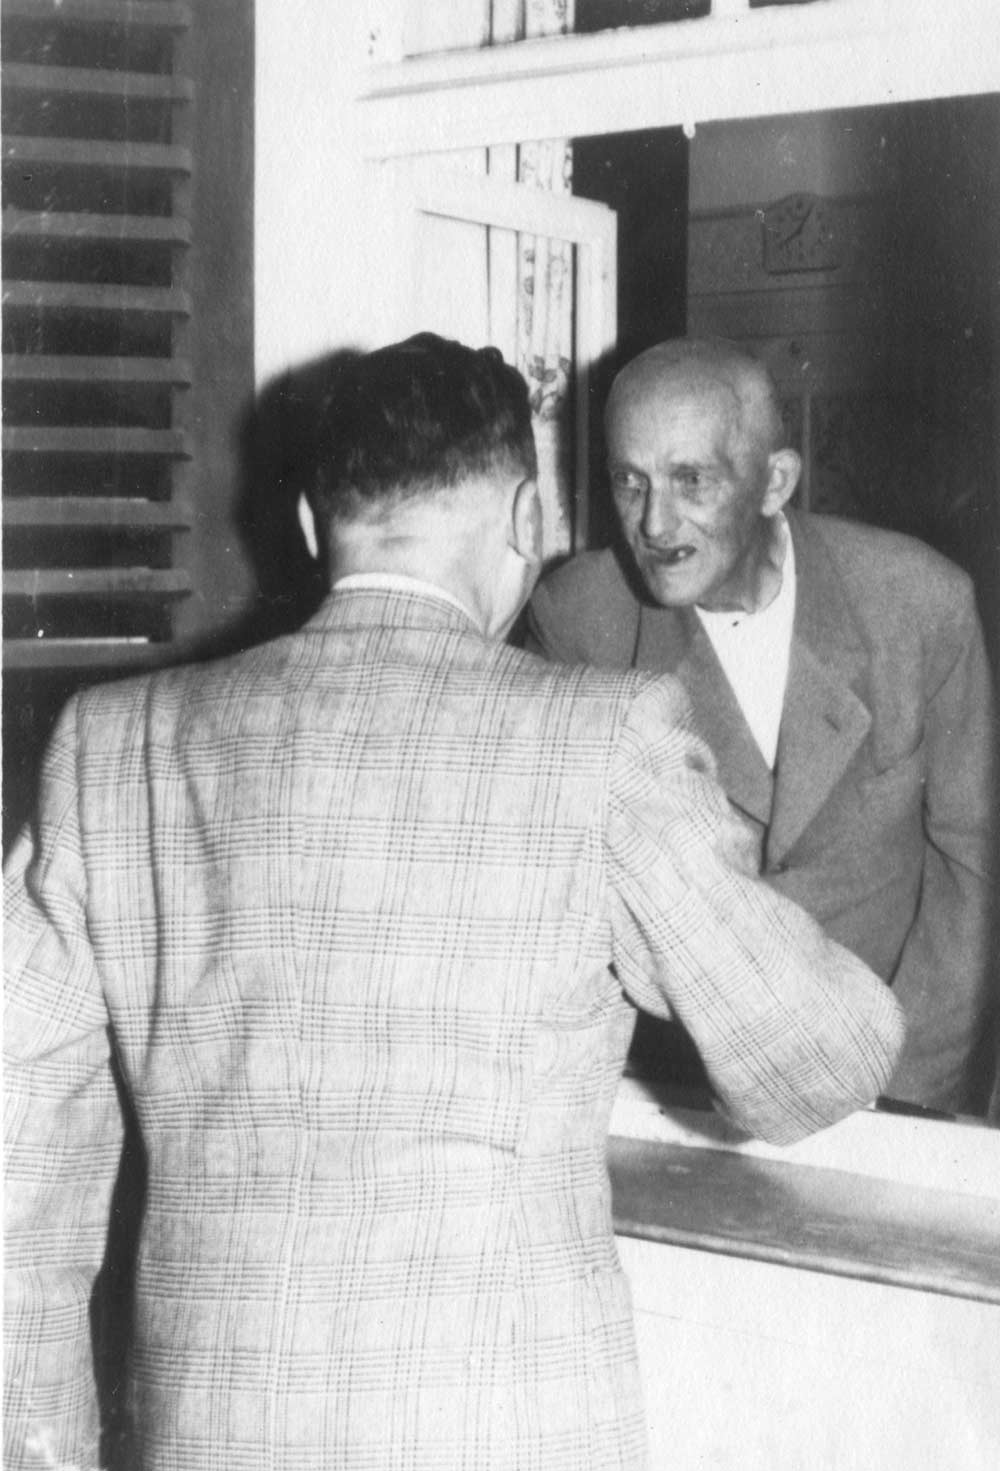
\includegraphics[width=4.128cm,height=6.071cm]{pictures/zulassungsarbeit-img054.jpg}

Franz Danziger gratuliert August Högn
am Vorabend zu seinem 80. Geburtstag &

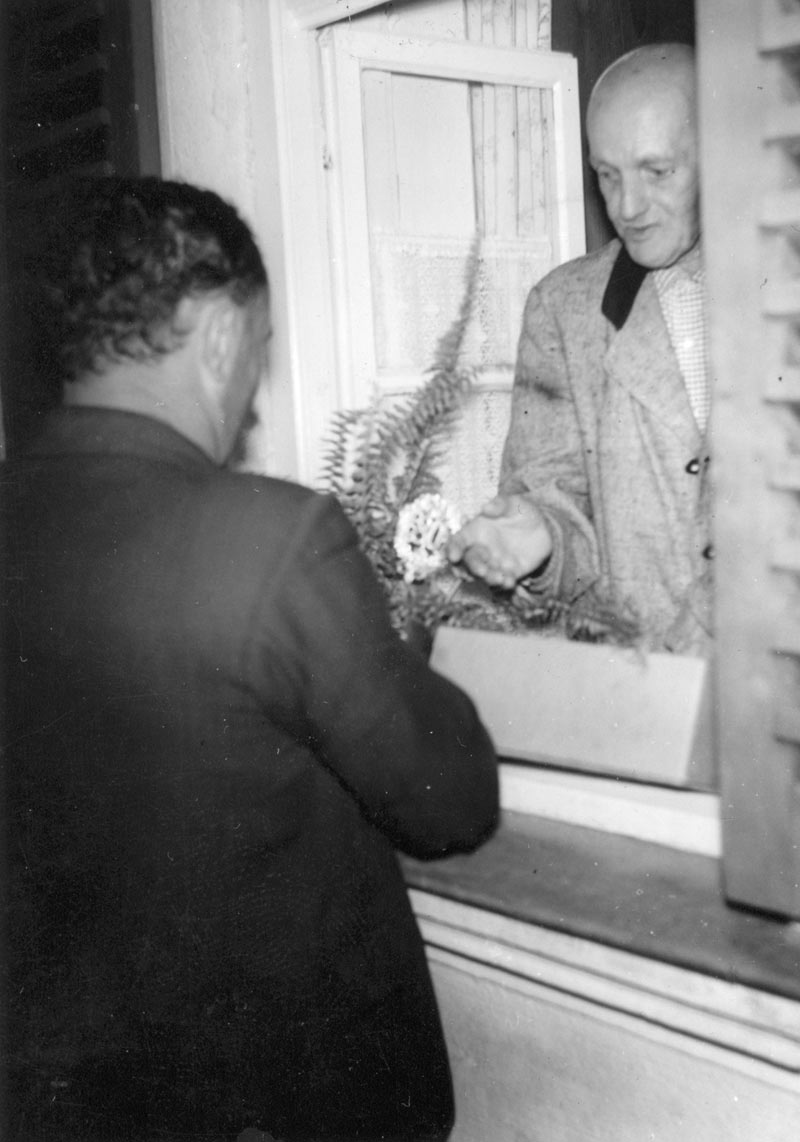
\includegraphics[width=4.255cm,height=6.073cm]{pictures/zulassungsarbeit-img055.jpg}

Der Zachenberger Bürgermeister
Bielmeier überreicht August Högn einen Geschenkkorb zum 80.
Geburtstag\\
\end{supertabular}
\end{center}
\end{minipage}
\end{center}
Ende 1960 scheint sich Högns Gesundheitszustand zu verschlechtern. Er
beklagt sich, dass das sein \zitat{„gesundheitliches Befinden
nicht das beste“} ist und das \zitat{„Marschieren sehr
schlecht geht.“ }Um Besserung zu erfahren, sucht er sogar einen Arzt im
mehr als 50 km entfernten Straubing auf. \footnote{Dokument Nr. 72,
Brief von August Högn an Stephan Leitner, Dez. 1960} Er ist immer mehr
auf Hilfe anderer angewiesen und seine Haushälterin Rosa Beischmied
wird zur \zitat{„Krankenfürsorgerin.“ } \footnote{Dokument
Nr. 73, Brief von August Högn an Stephan Leitner,
10.3.1961}Ein letztes Foto von Högn vom Juli
1961 zeigt zwar einen hageren, alten Mann, der an den Folgen seines
Schlaganfalles sichtbar leidet, doch es zeigt keinen vom Tode
gekennzeichneten Mann, der wenige Monate später sterben wird.

August Högn starb am 13. Dezember 1961 um 5 Uhr morgens.\footnote{
Dokument Nr. 50, Zeitungsartikel aus dem Viechtacher Bayerwald-Bote,
14.12.1961} Sein Tod kam nicht plötzlich, da er rechtzeitig mit den
Sterbesakramenten versehen worden war. \footnote{Dokument Nr. 50,
Zeitungsartikel aus dem Viechtacher Bayerwald-Bote, 14.12.1961} Nach
Aussagen von Högns Enkelin Gertraud von Molo war er bis kurz vor seinem
Tod rüstig \footnote{Interview Nr. 20, Gertraud von Molo, 23.11.2004,
Absatz 14} und sein Tod dürfte auf eine eher \zitat{„kürzere
Krankheit“ } \footnote{Interview Nr. 2, Barbara Essigmann, 27.12.2002,
Absatz 62} zurückzuführen sein, als auf eine \zitat{„lange
schwere“}  \footnote{Dokument Nr. 51, Zeitungsartikel aus Viechtacher
Bayerwald-Bote, 15.12.1961} Krankheit, wie es im seinem Nachruf im
Viechtacher Bayerwald-Boten steht. Im Sterberegister der Pfarrei
Ruhmannsfelden steht als Todesursache „Herzinsuffizienz“, was eher auf
einen plötzlichen Tod schließen lässt. \footnote{Dokument Nr. 112,
Eintrag im Sterberegister des Pfarramts Ruhmannsfelden, 13.12.1961}
Waren bei der Überführung des Leichnams am Todestag anwesend\footnote{
Dokument Nr. 51, Zeitungsartikel aus Viechtacher Bayerwald-Bote,
15.12.1961} nur wenige enge Freunde, die dem Leichenauto Richtung
Deggendorf einige hundert Meter folgten, \footnote{Interview Nr. 2,
Barbara Essigmann, 27.12.2002, Absatz 64} so dürfte es beim im
Ruhmannsfelden abgehaltenen Requiem am darauffolgenden Tag in
Ruhmannsfelden ein Großteil der Ruhmannsfeldener Bevölkerung gewesen
sein, der von Högn Abschied nahm. Die Ruhmannsfeldener Volksschule nahm
an der Trauerfeier teil und jeder ehemalige Schüler erhielt eine
Einladung zum Besuch des Trauergottesdienstes. \footnote{Dokument Nr.
50, Zeitungsartikel aus dem Viechtacher Bayerwald-Bote, 14.12.1961} Die
offizielle Beerdigung fand am 15. Dezember in der Deggendorfer
Pfarrkirche Mariä Himmelfahrt statt. \footnote{Dokument Nr. 66,
Todesbenachrichtigung, 13.12.1961} Bei eisiger Kälte\footnote{
Interview Nr. 3, Ida Högn, 29.12.2002, Absatz 20} hielten die Lehrer
Karl Schambeck, \footnote{Dokument Nr. 52, Brief von Elfriede
Schlumprecht an Lehrer Schambeck, 3.1.1962} Franz Nemetz\footnote{
Interview Nr. 3, Ida Högn, 29.12.2002, Absatz 20; Dokument Nr. 53,
Brief von Elfriede Schlumprecht an Rektor Langesee, 3.1.1962} und der
Kreisschulrat Botschafter \footnote{Dokument Nr. 53, Brief von Elfriede
Schlumprecht an Rektor Langesee, 3.1.1962} am Grab Trauerreden auf
August Högn. Besonders die Ansprache von Lehrer Nemetz blieb als eine
sehr lange Rede bei vielen Anwesenden in Erinnerung.\footnote{
Interview Nr. 3, Ida Högn, 29.12.2002, Absatz 20} Abordnungen der
Vereine aus Ruhmannsfelden waren mit Fahnen anwesend und eine
Bläsergruppe der freiwilligen Feuerwehr von Ruhmannsfelden spielte für
ihr Ehrenmitglied zum Abschied das Lied „Wir hatten einen Kameraden.“
 \footnote{Interview Nr. 20, Gertraud von Molo, 23.11.2004, Absatz 42}
August Högn fand seine letzte Ruhestätte auf dem Deggendorf Friedhof,
im schönen Grabmal \footnote{Interview Nr. 20, Gertraud von Molo,
23.11.2004, Absatz 10} neben seiner 1926 verstorbenen Ehefrau Emma.

\begin{center}
\begin{minipage}{5.542cm}
\begin{flushleft}
\tablefirsthead{}
\tablehead{}
\tabletail{}
\tablelasttail{}
\begin{supertabular}{m{5.342cm}}

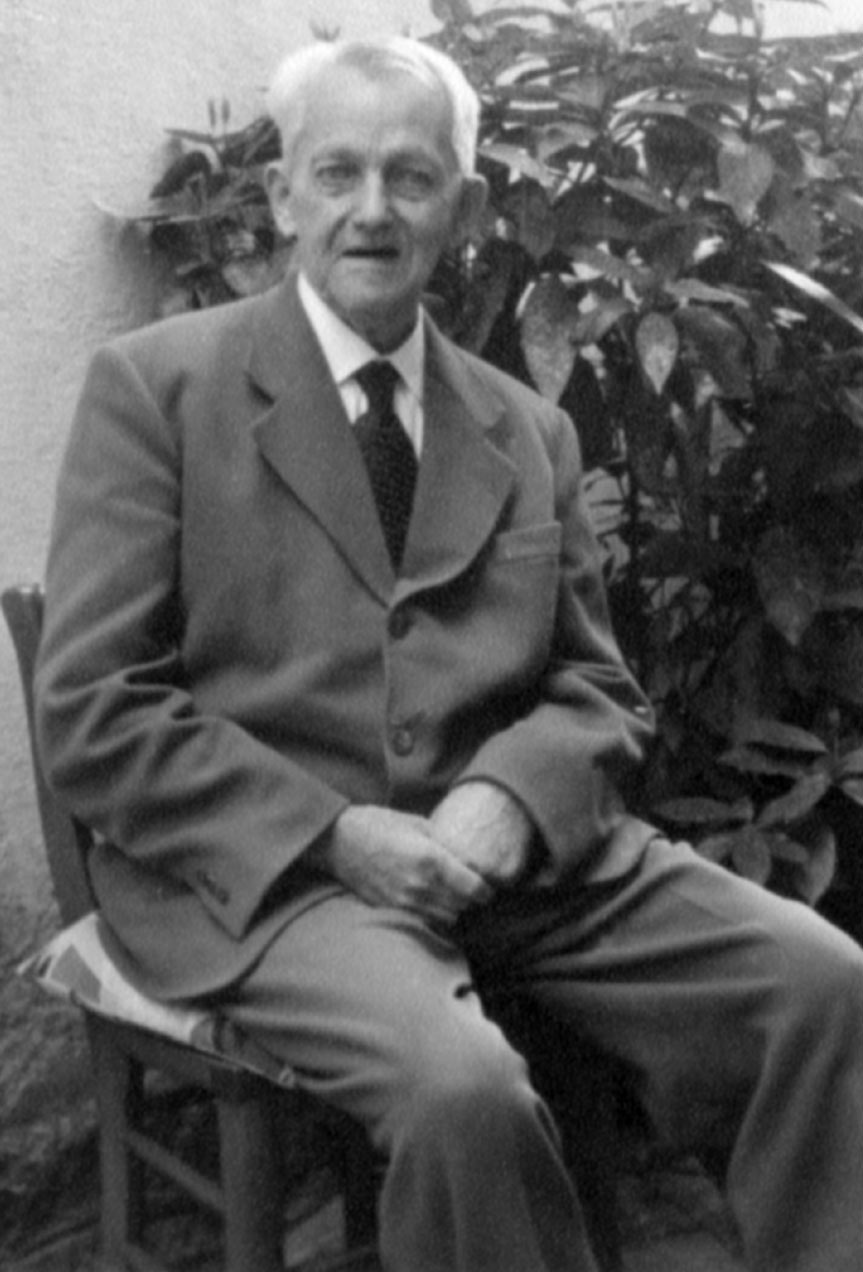
\includegraphics[width=5.159cm,height=7.606cm]{pictures/zulassungsarbeit-img056.jpg}

letztes Foto von August Högn, Juli
1961\\
\end{supertabular}
\end{flushleft}
\end{minipage}
\end{center}
\begin{flushleft}
\tablefirsthead{}
\tablehead{}
\tabletail{}
\tablelasttail{}
\begin{supertabular}{m{12.311cm}m{3.6929998cm}}

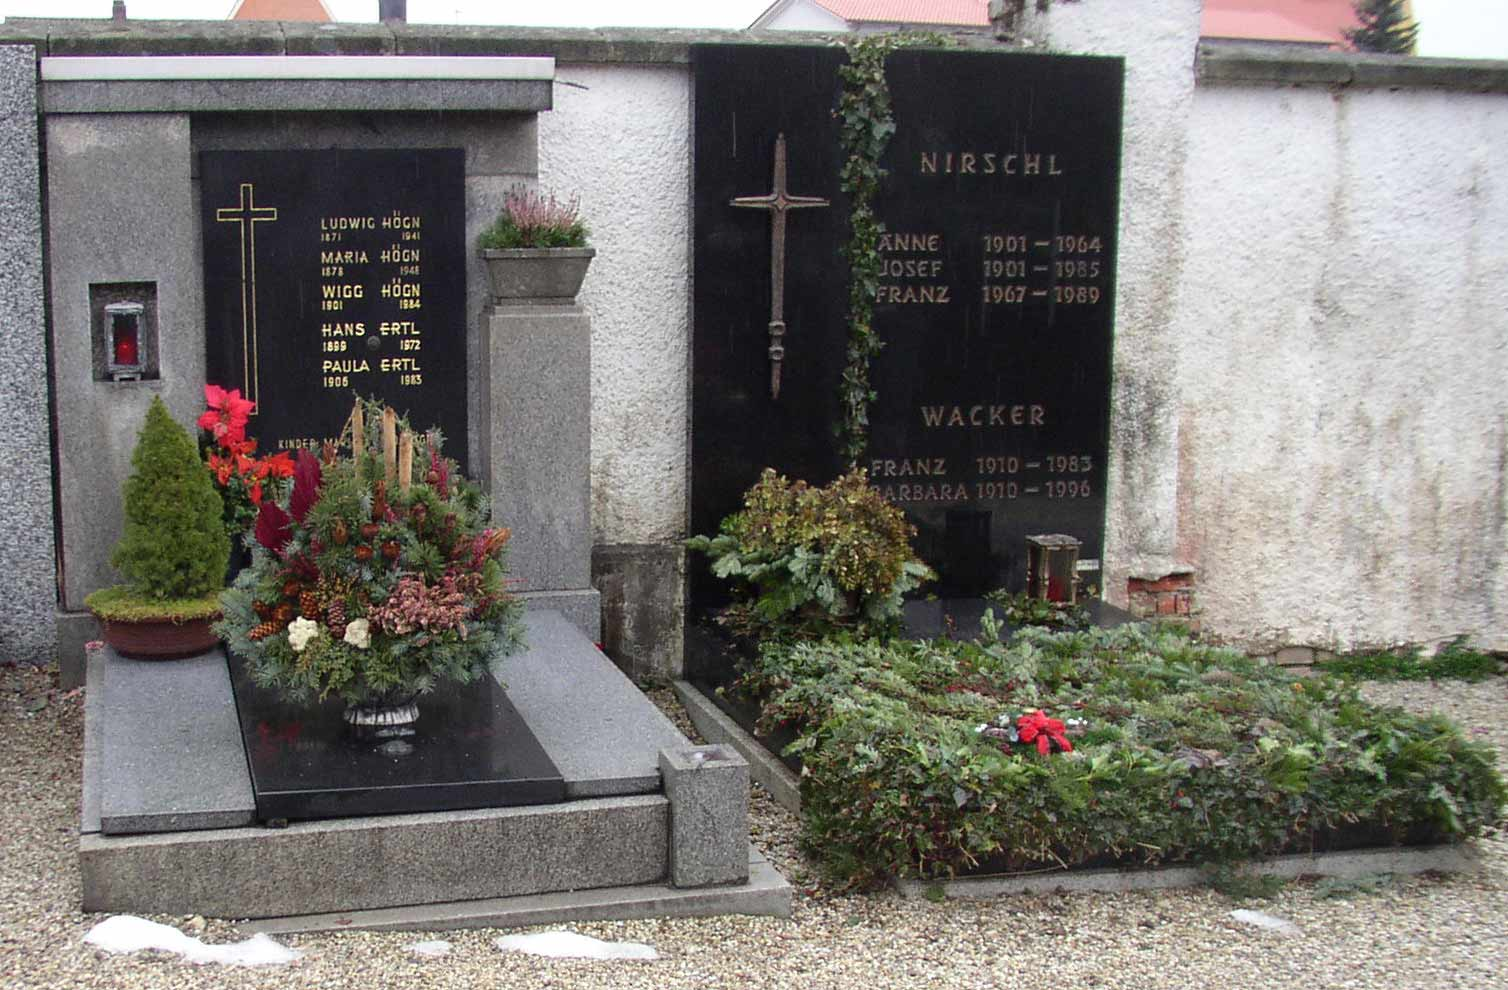
\includegraphics[width=12.129cm,height=8.015cm]{pictures/zulassungsarbeit-img057.jpg}

Familiengrab von Ludwig Högn (links)
und ehemalige Grabstätte von August Högn und seiner Ehefrau (rechts),
heute im Besitz der Familie Nirschl &

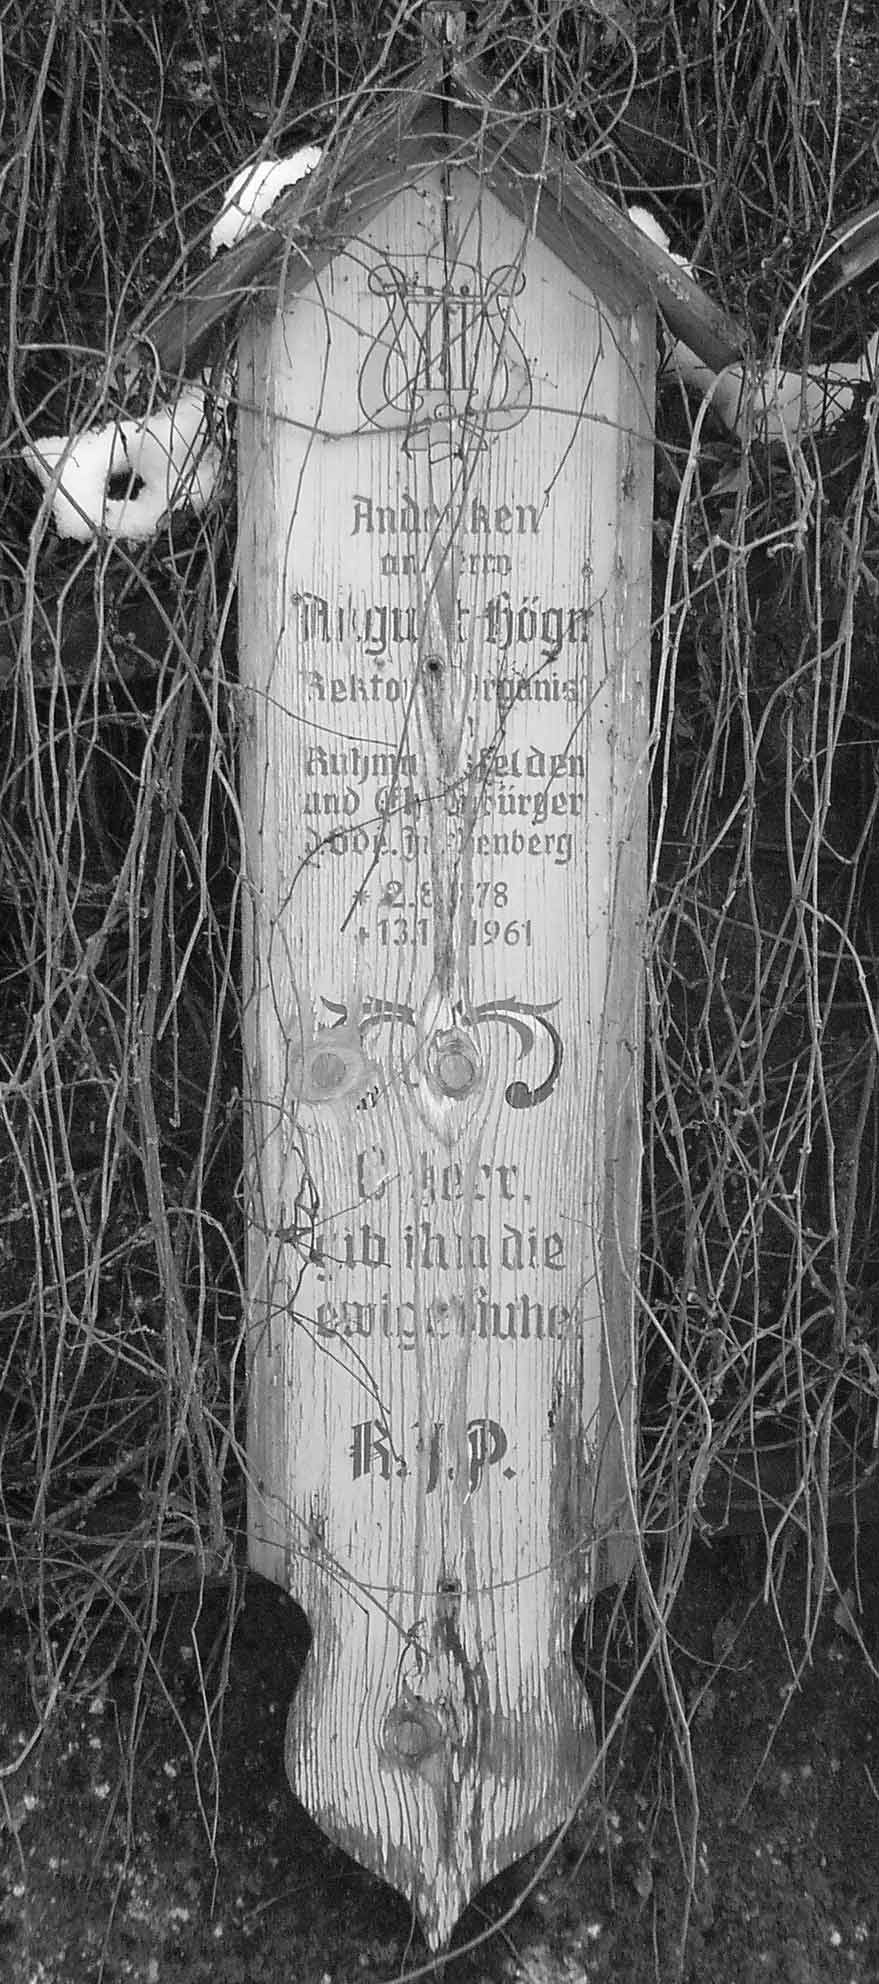
\includegraphics[width=3.51cm,height=7.978cm]{pictures/zulassungsarbeit-img058.jpg}

Totenbrett zum Andenken von August Högn
an der Wallfahrtskirche Osterbrünnl in Ruhmannsfelden\\
\end{supertabular}
\end{flushleft}
